\section{Introduction}
\label{sec:introduction}
One of the litanies about data management systems is that they are I/O
bound, i.e., limited in performance by the bandwidth to the primary
storage medium (be it disk or RAM). Indeed, many operations like scans
or aggregations are relatively easy to implement at sufficiently high
CPU-efficiency to make I/O bandwidth the dominating cost
factor. However, other operations like joins or index-building are
mostly bound by the computation speed of the CPU. When exploring
alternative algorithms for data management operations, it is crucial
to understand the contributing cost factors for the existing as well
as the new implementation.

\emph{Database Cracking} was introduced as an alternative to scanning
 to evaluate range-predicates on relational data. Rather than
copying the matching tuples into a result buffer, \emph{Cracking}
physically partitions the data in-place using the specified
range as pivot(s). Since one of the resulting partitions contains only the
qualifying tuples, \emph{Cracking} effectively answers the query. 
%As a side effect,
Additionally,
the reordered data can be combined with an appropriate
secondary data structure (usually a tree or a hash) to form a partial
clustered index. Assuming that the next query can benefit from such a
clustered index, the extra costs for the physical reordering will pay
off over time. 

Since the fix-point of \emph{Cracking} is fully sorted data, its
costs are usually compared to those of fully sorting the data. With
recent advancements in data (parallel) sorting
algorithms~\cite{sorting_SIMD}, however, \emph{Cracking} appears
increasingly unattractive. To illustrate this,
Figure~\ref{fig:motivation} shows a quick comparison of the respective
operations on 512 Million 32-bit integer values on a 4-Core
Sandy Bridge CPU.
%
\begin{figure}[t!]
  \centering
  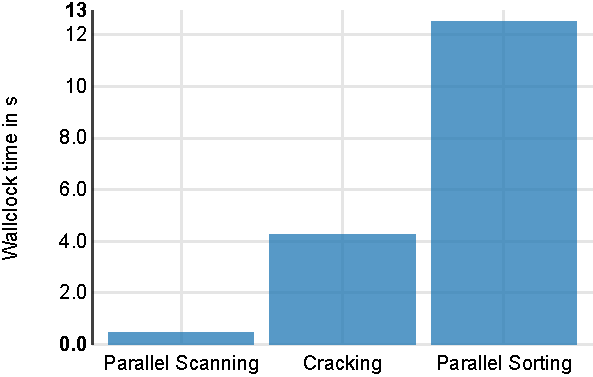
\includegraphics[width=.9\columnwidth]{Figures/damon/Motivation}
  \caption{Costs of Database Operations}
\vspace{-0.2 in}
  \label{fig:motivation}
\end{figure}
%
It shows that while an off-the-shelf \emph{(Parallel) Mergesort}
implementation\footnote{Part of the GNU libstdc++ Version 4.8.2} is
about 30 times more expensive than a (quasi I/O bound) \emph{(Parallel)
  Scan}, it is only three times as expensive as MonetDB's
implementation of \emph{Cracking}~\cite{DBLP:conf/cidr/IdreosKM07}.
Even though both \emph{Scanning} and \emph{Cracking},
(sequentially) read and write the same amount of data, they have
vastly different costs. The performance difference must, thus, be
due to their computational costs: \emph{Cracking}
is, unlike \emph{Scanning}, not I/O bound. However,\\[-2ex]
\begin{center}
  \begin{minipage}{.95\linewidth}
    \emph{we believe} that, if implemented with the underlying
    hardware in mind, \emph{Cracking} can be (roughly) I/O bound.
\end{minipage}
\end{center}
\vspace{1ex}
%
%
To validate this hypothesis, we make the following contributions:
\vspace{-1ex}
\begin{itemize}
  %\setlength{\itemsep}{0pt}
  %\setlength{\parskip}{0pt}
  %\setlength{\parsep}{0pt}
\item We conduct an in-depth study of the contributing performance factors
  of the ``classic'' \emph{Cracking} implementation.
\item Based on the findings, we develop a number of optimizations
  based on ``standard'' techniques like predication, vectorization and
  manually implemented data parallelism using SIMD instructions.
\item We develop two different parallel algorithms that exploit thread
  level parallelism to make use of multiple CPU cores.
\item We rigorously evaluate all developed algorithms on a number of
  different systems ranging from low-end desktop machines to high-end
  servers.
\end{itemize}
\vspace{-1ex}

The rest of the paper is structured as follows: In
Section~\ref{sec:related-work}, we provide an overview of related work
as well as necessary background knowledge on the optimization
techniques we applied. In Section~\ref{sec:classic-cracking} we
present our analysis of the \emph{Cracking} implementation in MonetDB
discussing its problems with regard to CPU efficiency.
We present our CPU-optimized sequential \emph{Cracking} algorithms
in Section~\ref{sec:cracking-algorithms},
and our parallel implementations in Section~\ref{subsec:tlp}.
We evaluate these algorithms on a range of different
hardware platforms in Section~\ref{sec:results} and conclude in
Section~\ref{sec:conclusion}.

